\documentclass[11pt,a4paper]{article}
\usepackage[a4paper,hmargin=1in,vmargin=1in]{geometry}
\usepackage{pgfplots}
\pgfplotsset{compat=1.17}

\usepackage[czech]{babel}
\usepackage[utf8]{inputenc}
\usepackage[T1]{fontenc}

\usepackage[nodayofweek]{datetime}
\newdate{date}{14}{6}{2023}

\usepackage{stddoc}
\usepackage{lipsum}
\usepackage{subcaption}
% \usepackage[square,numbers]{natbib}
% \usepackage[nottoc]{tocbibind}

\newcommand{\plus}{{\texttt{+}}}
\renewcommand{\Re}{\operatorname{Re}}
\renewcommand{\Im}{\operatorname{Im}}
\newcommand{\fourier}[3]{\mathcal{F}_{#1}\!\left[#2\right]\!\left(#3\right)}
\newcommand{\ifourier}[3]{\mathcal{F}^{-1}_{#1}\!\left[#2\right]\!\left(#3\right)}
\newcommand{\dB}{\mathrm{dB}}
\newcommand{\dBm}{\mathrm{dBm}}
\newcommand{\MHz}{\mathrm{MHz}}
\newcommand{\GHz}{\mathrm{GHz}}
\newcommand{\kHz}{\mathrm{kHz}}


\begin{document}

\pagenumbering{arabic}

% Header
\begin{center}
    {\LARGE\textbf{Laboratorní úloha č. 11}}\\[3mm]
    \begin{minipage}{0.4\textwidth}
        \begin{flushleft}
            \textsc{\displaydate{date}}
        \end{flushleft}
    \end{minipage}
    ~
    \begin{minipage}{0.4\textwidth}
        \begin{flushright}
            \textsc{Martin Šimák}
        \end{flushright}
    \end{minipage}
    \noindent\rule{14.5cm}{0.4pt}
\end{center}

\paragraph*{Měření permitivity materiálů} Laboratorní úloha ukazuje využití vektorového měření pro určování frekvenčního průběhu efektivní i relativní permitivity různých materiálů.

\subsection*{Úkoly měření}
\begin{enumerate}
    \item Měření frekvenčního průběhu efektivní permitivity mikropáskového vedení pomocí přímkového 
    rezonátoru.
    \item Měření frekvenčního průběhu efektivní permitivity mikropáskového vedení pomocí prstencového rezonátoru.
    \item Měření relativní permitivity materiálu ABS ve vlnovodu.
\end{enumerate}

\subsection*{Použité přístroje a komponenty}
\begin{itemize}
    \item Vektorový analyzátor R\&S ZVA67 (10~MHz až 67~GHz)
    \item Elektronická kalibrační jednotka R\&S ZV-Z52 (10~MHz až 24~GHz)
\end{itemize}

\subsection*{Popis měření}

% Task 1
\paragraph*{Měření frekvenčního průběhu efektivní permitivity mikropáskového vedení pomocí přímkového rezonátoru} Subjektem měření je mikropáskové vedení šířky 0.7~mm a délky 34~mm, které je umístěno do kovové krabičky a má otevřené konce, které jsou jen přiblížené k pinům SMA konektorů. Použitý substrát je CuClad\textregistered\ 233 od firmy Rogers s tloušťkou 0.254~mm. Podél délky vedení $L$ je možné rozmístit celé násobky $\lambda/2$ stojaté vlny, která má kmitny elektrického pole na otevřených koncích vedení. Vlnová délka na mikropáskovém vedení je dána vztahem
\begin{align}
    \lambda &= \frac{c}{f\sqrt{\epsilon_{\mathrm{eff}}}},
\end{align}
kde $c$ je rychlost světla a $\epsilon_{\mathrm{eff}}$ je efektivní permitivita vedení.

Pro nastavení vektorového analyzátoru volíme frekvenční pásmo 20~MHz až 24~GHz a výkon 0~dBm. Dále počet frekvenčních bodů volíme tak, aby byl frekvenční krok měření 20~MHz. Šířku pásma mezifrekvenčního filtru RBW je vhodné volit tak, aby měření probíhalo za akceptovatelný čas, ale abychom zároveň dosáhli dostatečné šumové separace. Kalibraci provádíme pomocí automatické kalibrační jednotky, která umožňuje velice přesnou kalibraci s dobrou opakovatelností. Exportované grafy modulu a fáze S-parametrů vedení jsou na obrázku~\ref{fig:primkovy-rezonator}.
\begin{figure}[!ht]
\centering
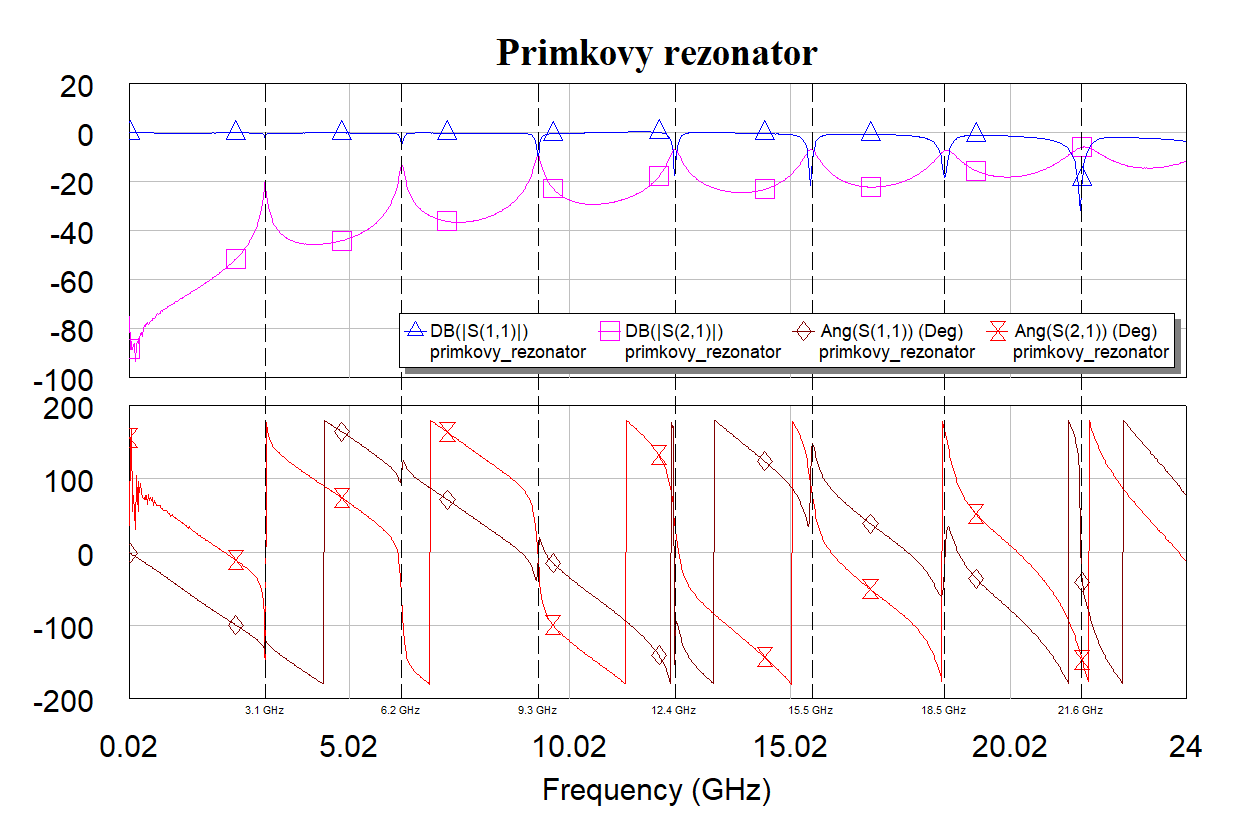
\includegraphics[width=.9\textwidth]{src/primkovy-rezonator.png}
\caption{Modul a fáze vedení s přímkovým rezonátorem}
\label{fig:primkovy-rezonator}
\end{figure}

Pro všechny odečtené rezonanční frekvence jsou vypočtené hodnoty permitivity zaneseny v tabulce~\ref{table:primkovy-rezonator} a jejich průběh graficky znázorněn na obrázku~\ref{fig:primkovy-rezonator-permitivita}. Zpracování bylo provedeno formou porovnání vlnové délky ve volném prostoru ($\lambda_0 = c/f$) s délkou měřeného vedení tak, aby jednotlivé rezonance odpovídaly rovnosti
\begin{align}
    L &= m\lambda/2,
\end{align}
kde $m \in \N$. Očividnou diskuzí je volba násobku $m$ vlnové délky pro první zobrazovanou rezonanci, ale jelikož pro volbu $m=1$ vychází frekvenční disperze permitivity v rámci očekávatelných mezí, byla posouzena jako správná.
\begin{table}[!ht]
    \centering
    \begin{tabular}{|l||c|c|c|c|c|c|c|}
        \hline
        $f_{\mathrm{res}}\ [\GHz]$ & 3.1 & 6.2 & 9.3 & 12.4 & 15.5 & 18.5 & 21.6\\
        \hline
        $\epsilon_{\mathrm{eff}}\ \[-\]$ & 2.03 & 2.03 & 2.03 & 2.03 & 2.03 & 2.05 & 2.04\\
        \hline
    \end{tabular}
    \caption{\label{table:primkovy-rezonator}Zjištěné hodnoty permitivity vedení s přímkovým rezonátorem}
\end{table}
\begin{figure}[!ht]
\centering
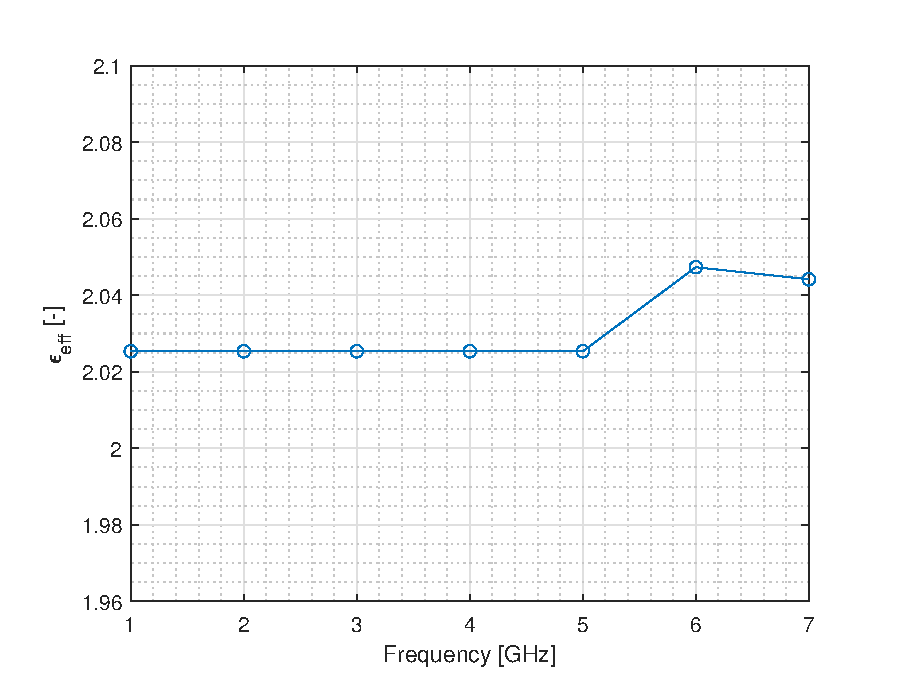
\includegraphics[width=.6\textwidth]{src/primkovy-rezonator-permitivita.eps}
\caption{Přímkový rezonátor -- grafické znázornění}
\label{fig:primkovy-rezonator-permitivita}
\end{figure}

% Task 2
\paragraph*{Měření frekvenčního průběhu efektivní permitivity mikropáskového vedení pomocí prstencového rezonátoru} Měřeným vedením v této úloze je přípravek s prstencovým rezonátorem. Tento přípavek je vyroben na substrátu Rogers RO4003C s tloušťkou 0.508 mm. Šířka vedení prstence je 0.7 mm a vnější průměr je 34 mm. Průběh S-parametrů, z něhož čteme rezonanční frekvence, je na obrázku~\ref{fig:prstencovy-rezonator}.
\begin{figure}[!ht]
\centering
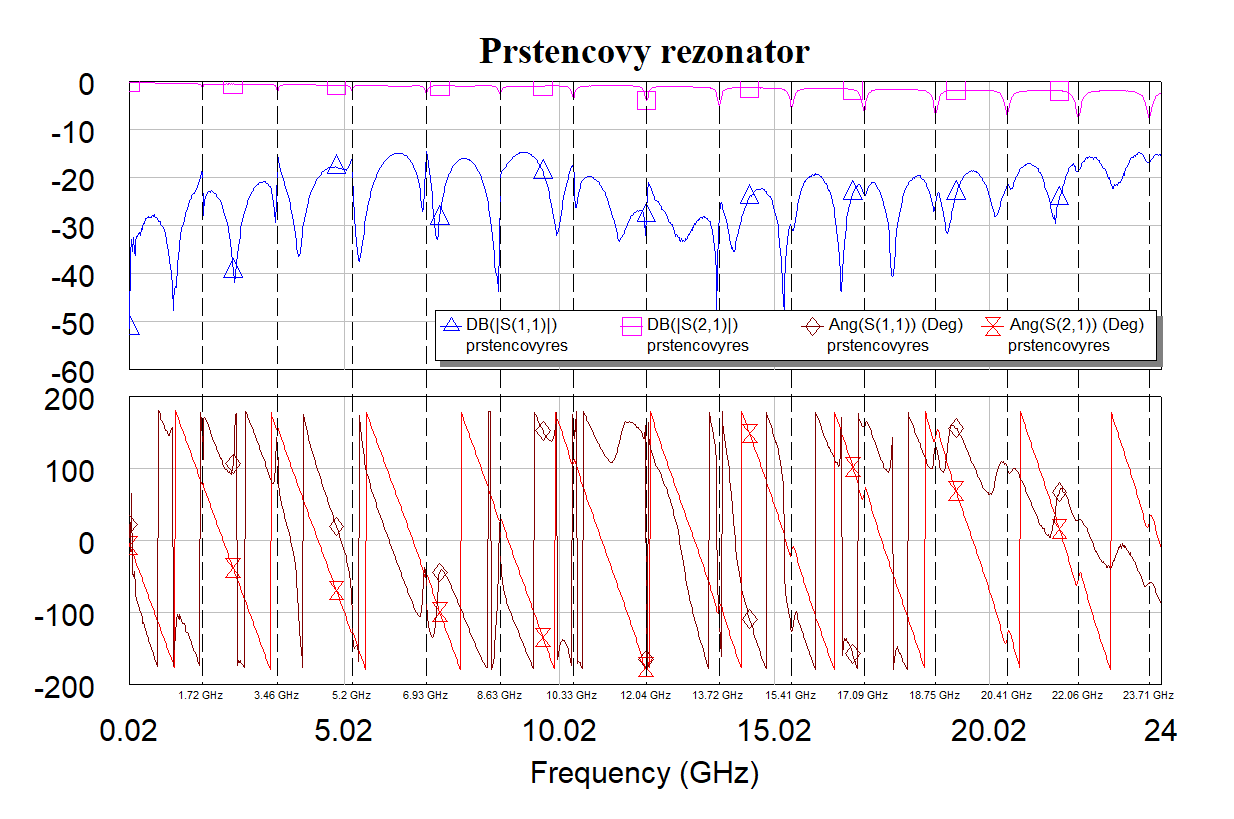
\includegraphics[width=\textwidth]{src/prstencovy-rezonator.png}
\caption{Modul a fáze vedení s prstencovým rezonátorem}
\label{fig:prstencovy-rezonator}
\end{figure}

Pro všechny odečtené rezonanční frekvence jsou vypočtené hodnoty permitivity zaneseny v tabulce~\ref{table:prstencovy-rezonator} a jejich průběh graficky znázorněn na obrázku~\ref{fig:prstencovy-rezonator-permitivita}. Zpracování bylo provedeno formou porovnání vlnové délky ve volném prostoru s vnějším průměrem rezonátoru tak, aby jednotlivé rezonance odpovídaly rovnosti
\begin{align}
    2\pi\(R-\frac w2\) &= m\lambda,
\end{align}
kde $m \in \N$, $R$ je vnější průměr a $w$ je šířka pásku rezonátoru.
\begin{table}[!ht]
    \centering
    \begin{tabular}{|l||c|c|c|c|c|c|c|}
        \hline
        $f_{\mathrm{res}}\ [\GHz]$ & 1.72 & 3.46 & 5.2 & 6.93 & 8.63 & 10.33 & 12.04\\
        \hline
        $\epsilon_{\mathrm{eff}}\ \[-\]$ & 2.72 & 1.51 & 1.19 & 1.05 & 0.97 & 0.92 & 0.89\\
        \hline\hline
        $f_{\mathrm{res}}\ [\GHz]$ & 13.72 & 15.41 & 17.09 & 18.75 & 20.41 & 22.06 & 23.71\\
        \hline
        $\epsilon_{\mathrm{eff}}\ \[-\]$ & 0.87 & 0.85 & 0.83 & 0.82 & 0.82 & 0.81 & 0.81\\
        \hline
    \end{tabular}
    \caption{\label{table:prstencovy-rezonator}Zjištěné hodnoty permitivity vedení s přímkovým rezonátorem}
\end{table}
\begin{figure}[!ht]
\centering
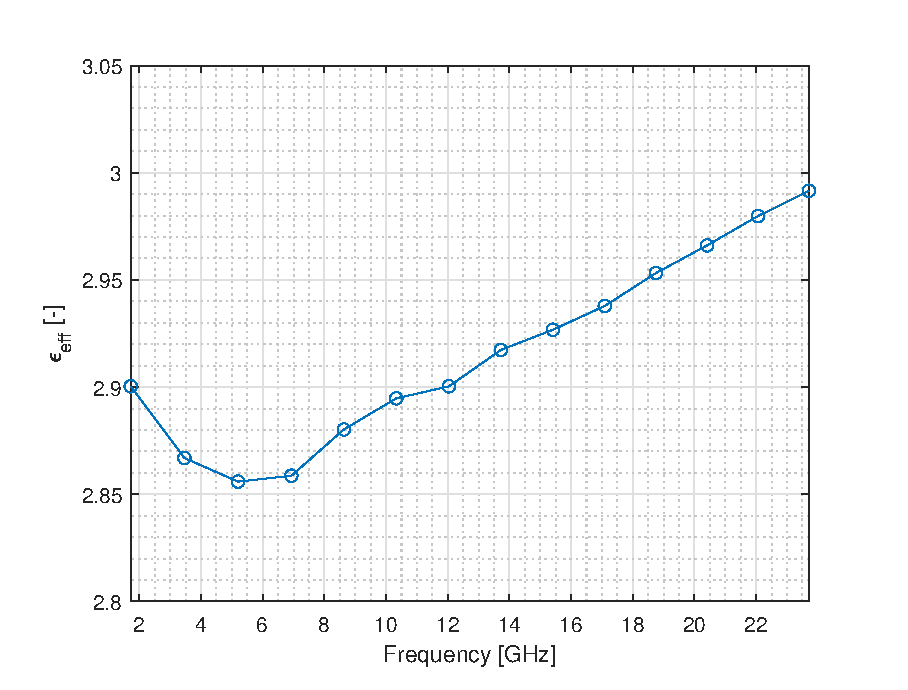
\includegraphics[width=.6\textwidth]{src/prstencovy-rezonator-permitivita.eps}
\caption{Prstencový rezonátor -- grafické znázornění}
\label{fig:prstencovy-rezonator-permitivita}
\end{figure}

% Task 3
\paragraph*{Měření relativní permitivity materiálu ABS ve vlnovodu} Pro měření na vlnovodu R100 je nutné upravit frekvenční pásmo na jednovidové pásmo vlnovodu (8.2~GHz až 12.4~GHz) a provést příslušnou kalibraci TRL. Pro kalibraci připojujeme mezi vlnovodné přechody rovné úseky vlnovodu vyplněné kvádry materiálu ABS vytisknuté na 3D tiskárně. Pro každý vzorek ukládáme frekvenční průběh změřených S-parametrů ve formátu Touchstone a následně analyzujeme v softwaru AWR.

Analýza v AWR probíhá tak, že si nejprve sestavíme ekvivalentní obvodové schéma jako je na obrázku~\ref{fig:r100-schematic}. Pro ostatní délky postupujeme analogicky. Proměnné $\mathit{ER}$ a $\mathit{TAND}$ jsou hodnoty efektivní permitivity $\epsilon_{\mathrm{eff}}$ a ztrátového faktoru $\tan(\delta)$, které jsou předmětem následné optimalizace.
\begin{figure}[!ht]
    \centering
    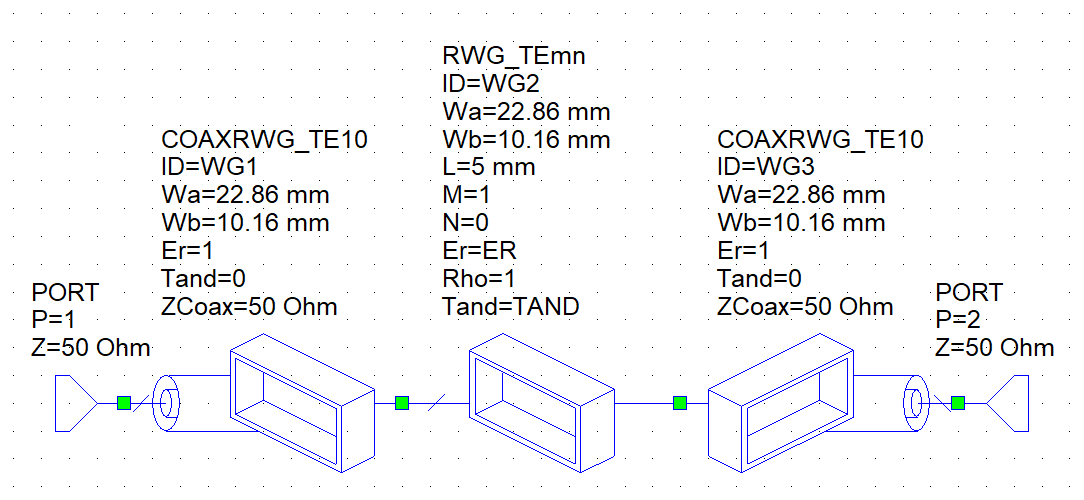
\includegraphics[width=.7\textwidth]{src/r100-schematic.png}
    \caption{\label{fig:r100-schematic}Ekvivalentní obvodové schéma vlnovodu R100 pro délku 5 mm}
\end{figure}

Dále v grafech sledujeme podobnost vypočítaných S-parametrů s importovanými průběhy z VNA, jak je vidět na obrázcích ve fig.~\ref{fig:r100-grafy}. Tuto podobnost maximalizujeme pomocí optimalizace proměnných $\mathit{ER}$ a $\mathit{TAND}$ simplexových algoritmem s cílem minimalizace kvadratické chybové funkce pro $S_{11}$ a $S_{21}$. Tyto rovnice sestavíme a optimalizujeme proměnné pro všechny čtyři konfigurace. Výsledné hodnoty jsou zaneseny v tabulce~\ref{table:vysledky-optimalizace}.
\begin{table}[!ht]
    \centering
    \begin{tabular}{|l||c|}
        \hline
        $\epsilon_{\mathrm{eff}}$ & $2.49$\\
        \hline
        $\tan(\delta)$ & $0.0024$\\
        \hline
    \end{tabular}
    \caption{\label{table:vysledky-optimalizace}Výsledky optimalizace}
\end{table}
\begin{figure}[!ht]
    \centering
\begin{subfigure}{0.45\textwidth}
    \centering
    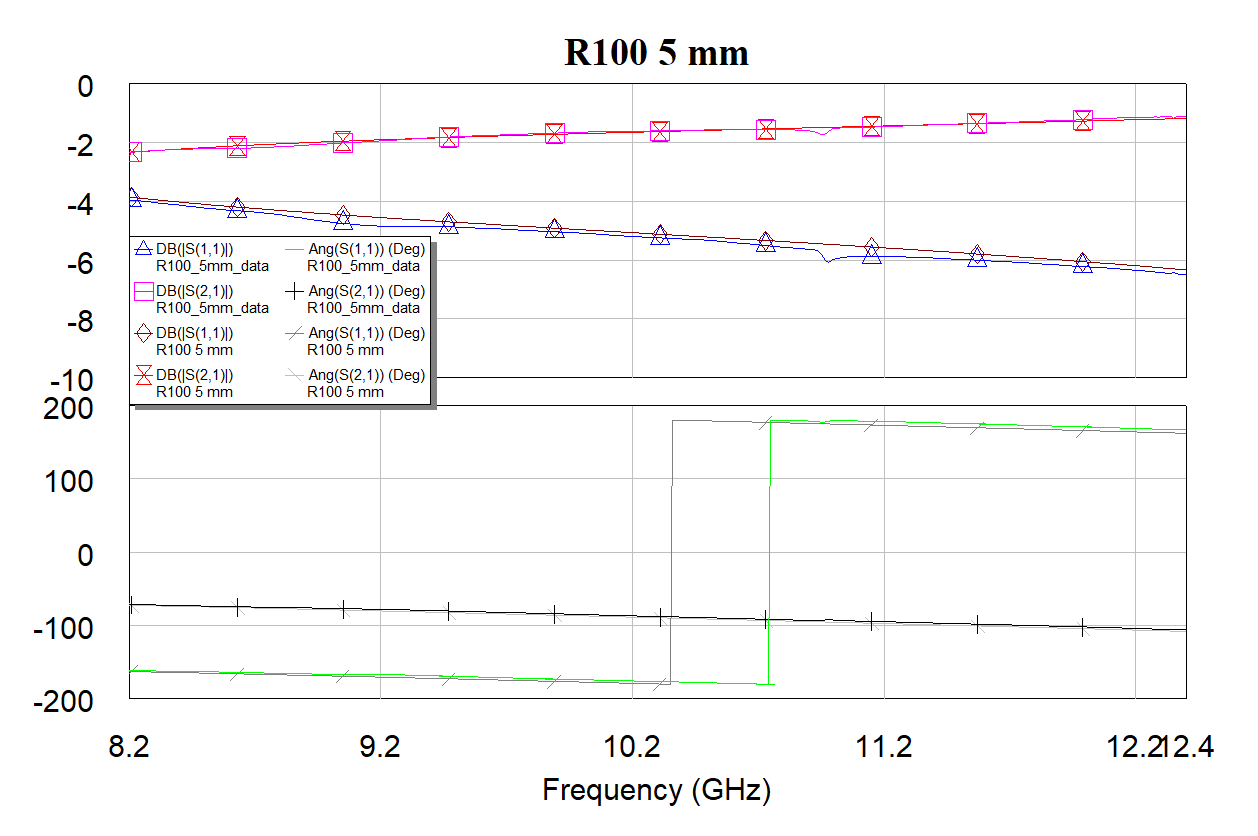
\includegraphics[width=\textwidth]{src/r100-5mm.png}
\end{subfigure}
\begin{subfigure}{0.45\textwidth}
    \centering
    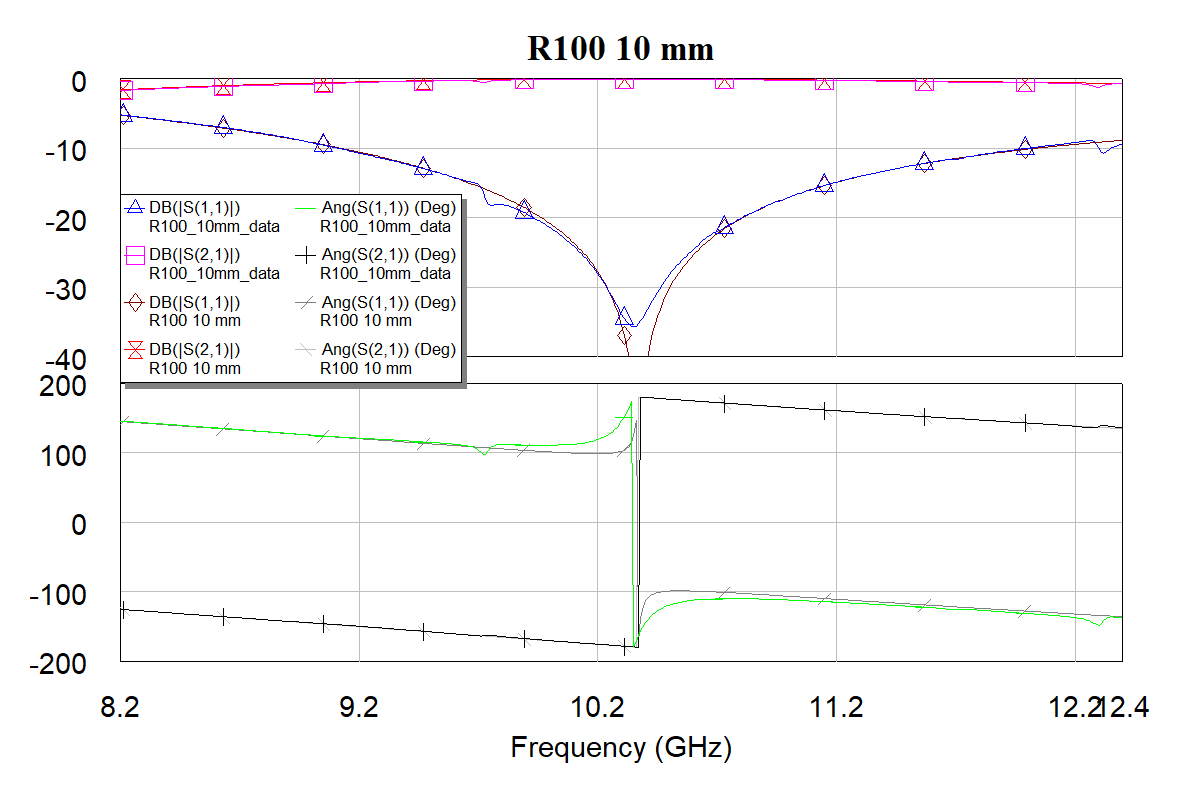
\includegraphics[width=\textwidth]{src/r100-10mm.png}
\end{subfigure}\\
\begin{subfigure}{0.45\textwidth}
    \centering
    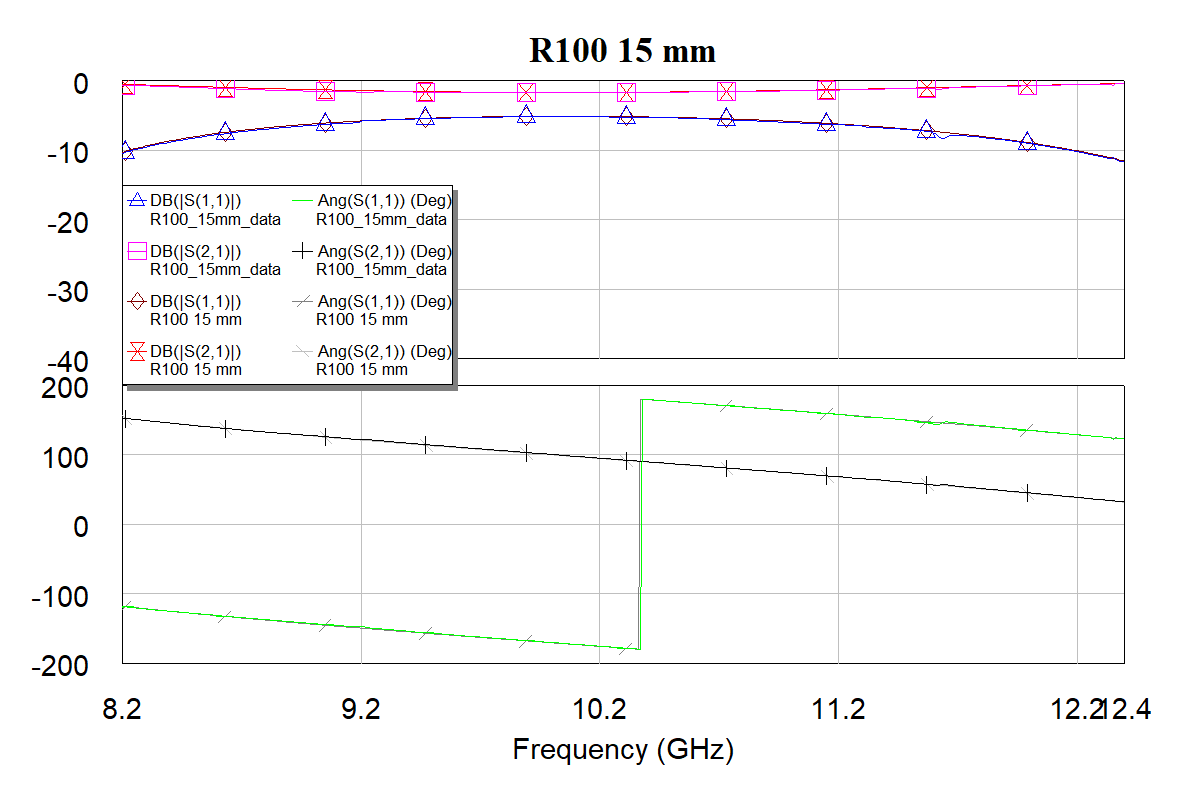
\includegraphics[width=\textwidth]{src/r100-15mm.png}
\end{subfigure}
\begin{subfigure}{0.45\textwidth}
    \centering
    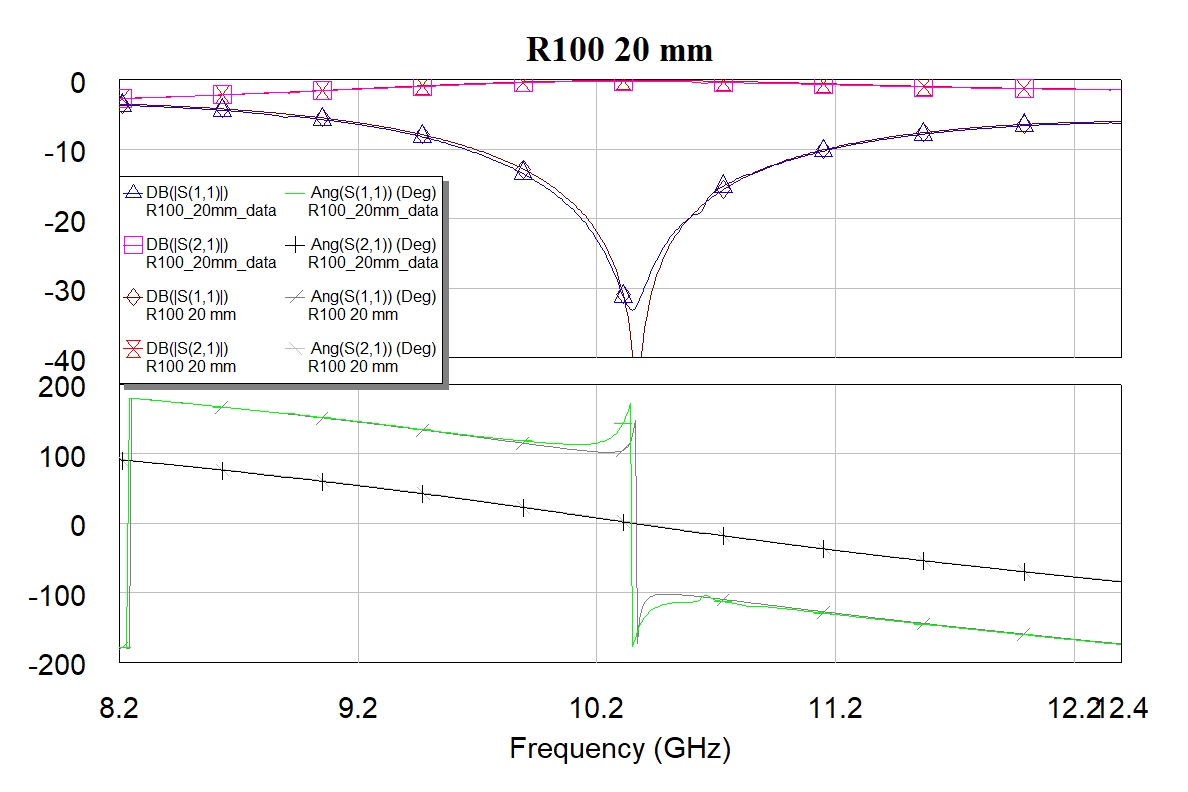
\includegraphics[width=\textwidth]{src/r100-20mm.png}
\end{subfigure}
\caption{\label{fig:r100-grafy}Modul a fáze vedení s úseky vlnovodu R100 různých délek}
\end{figure}

\subsection*{Závěr}
V rámci laboratorní úlohy jsme se seznámili s měřením efektivní permitivity pomocí tří různých metod, každá z nichž využívala jiné struktury vedení. První dvě metody využívaly rezonančního mikropáskového vedení a třetí vlnovod R100.  Měření proběhlo bez výraznějších potíží.

\end{document}
